% Name: Doubly linked list
% Description: Four nodes that each hold a value between a pointer back to the previous node and a pointer on to the next, with head and tail pointers and the two null ends crossed out.
% Tags: doubly linked list, pointers, nodes, data structures

\usetikzlibrary{arrows.meta}

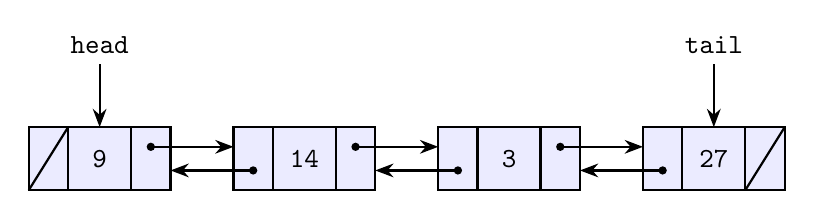
\begin{tikzpicture}[>={Stealth}, thick, every node/.style={font=\ttfamily}]
  % Node i spans x = 2.6i to 2.6i + 1.8: a prev cell, a value cell, and a next cell
  \foreach \v [count=\i from 0] in {9, 14, 3, 27} {
    \pgfmathsetmacro\x{2.6*\i}
    \draw[fill=blue!8] (\x,0) rectangle ++(1.8,0.8);
    \draw (\x+0.5,0) -- ++(0,0.8) (\x+1.3,0) -- ++(0,0.8);
    \node at (\x+0.9,0.4) {\v};
    \coordinate (n\i) at (\x,0);
  }
  % next pointers run along the top, prev pointers along the bottom
  \foreach \i in {0,1,2} {
    \pgfmathsetmacro\x{2.6*\i}
    \fill (\x+1.55,0.55) circle (1.5pt);
    \draw[->] (\x+1.55,0.55) -- (\x+2.6,0.55);
    \fill (\x+2.85,0.25) circle (1.5pt);
    \draw[->] (\x+2.85,0.25) -- (\x+1.8,0.25);
  }
  \draw (0,0) -- (0.5,0.8) (7.8+1.3,0) -- (7.8+1.8,0.8);
  \node[above=8mm] (head) at (0.9,0.8) {head};
  \node[above=8mm] (tail) at (7.8+0.9,0.8) {tail};
  \draw[->] (head) -- (0.9,0.8);
  \draw[->] (tail) -- (8.7,0.8);
\end{tikzpicture}
